\documentclass{article}
\usepackage{amsmath, amsthm, amssymb, amsfonts, bm}
\usepackage{graphicx}
\usepackage[T1]{fontenc}
\usepackage[utf8]{inputenc}
\usepackage[a4paper]{geometry}
\usepackage{fancyhdr}
\usepackage[algo2e]{algorithm2e}
%\usepackage{verbatim}
%\usepackage{framed}
%\usepackage{fancyvrb}
%\usepackage[dvipsnames]{xcolor}  % colors
\fontfamily{cmr}

%% redefine \VerbatimInput
%\RecustomVerbatimCommand{\VerbatimInput}{VerbatimInput}%
%{fontsize=\tiny,
% %
% frame=lines,  % top and bottom rule only
% framesep=1em, % separation between frame and text
% rulecolor=\color{Black},
% %
% label=\fbox{\color{Black}Synthesized text},
% labelposition=topline,
% %
% commandchars=\|\(\), % escape character and argument delimiters for
%                      % commands within the verbatim
% commentchar=*        % comment character
%}

\title{DD2424 - Assignment 4 (Bonus)}
\author{Oskar Stigland \\ stigland@kth.se}

\pagestyle{fancy}
\fancyhf{}
\rhead{stigland@kth.se}
\lhead{DD2424 - Deep Learning in Data Science}
\rfoot{Page \thepage}

\begin{document}
%\maketitle

	\begin{titlepage}
		\begin{center} 
			
			\rule{\linewidth}{0.5mm}\\[0.5 cm]
			{ \huge \bfseries DD2424 - Assignment 4 (Bonus)}\\[0.3 cm] % Title of your document
			\rule{\linewidth}{0.5mm}\\[1 cm]
					
			\small\vfill
			\begin{center}
			\centering
			{\large \bfseries \textsc{Summary}}\\
			\vspace{1cm}
			\begin{minipage}{10cm}
				
				I have completed three of the four suggested bonus extensions, using \texttt{Adam} instead of \texttt{Adagrad}, splitting the into chunks and randomizing them during training, and finally implementing temperature and nucleus sampling to attempt to generate more realistic text.\\\\
%
	The code for the assignment has been written in \texttt{python}. I have implemented the neural network as a class. For the hand-in, all of the code has been put toghether in a main file with all the functions and the class declared at the top. For the hand-in, I have also commented out the saving of generated figures and results in JSON files, as well as omitting some of the case-specific testing and gradient testing.
			\end{minipage}
			\end{center}
			\large\vfill
						

		\end{center}	
		
		\begin{minipage}{0.4\textwidth}
			\begin{flushleft} \large
				%\emph{Student:}\\
				Oskar \textsc{Stigland}\\
				DD2424\\
				Spring 2023
			\end{flushleft}
		\end{minipage}	

	\end{titlepage}

\newpage
\subsection*{\texttt{Adagrad} versus \texttt{Adam}}
	I first ventured into testing the effect of replacing the \texttt{Adagrad} optimizer with the much-popular \texttt{Adam}, for which we compute the updates as
	\begin{align*}
		\bm{w}_{k+1} &= \bm{w}_k - \eta\frac{\tilde{\bm{m}}_k}{\tilde{\bm{v}}_k + \epsilon} \\
		\tilde{\bm{m}}_k &= \bm{m}_k \times (1 - \beta_1^t + \epsilon)^{-1} \\
		\tilde{\bm{v}}_k &= \bm{v}_k \times (1 - \beta_2^t + \epsilon)^{-1} \\
		\bm{m}_k &= \beta_1^t \times \bm{m}_{k-1} + (1 - \beta_1^t)\times\nabla_{\bm{w}}L \\
		\bm{v}_k &= \beta_2^t \times \bm{v}_{k-1} + (1 - \beta_2^t) \times (\nabla_{\bm{w}}L)^2
	\end{align*}
	where $\epsilon$ is a very small numnber and $t$ is usually updated per training batch. Further, we have that $\beta_1 = 0.9$ and $\beta_2 = 0.999$. In this case, I have used $\eta = 0.01$ for both \texttt{Adagrad} and \texttt{Adam}, and since the data will be split into randomized chunks, $t$ is updated after each chunk, usually corresponding to some $500$ training examples. In order to properly check the effect of changing optimizer, I have also carved out the last $5$\% of the training examples for validation, and a smooth validation loss is tracked along with the smooth training loss. For the former, a random sample is selected after each training example and both smooth loss are then updated according to:
	    $$\tilde{\ell}^{\text{train}}_t = 0.999\times\tilde{\ell}^{\text{train}}_{t-1} + 0.001 \times\ell^{\text{train}}_{t}, \quad\text{and}\quad \tilde{\ell}^{\text{val}}_t = 0.999\times\tilde{\ell}^{\text{val}}_{t-1} + 0.001 \times\ell^{\text{val}}_{t}$$
	The difference in training performance when using \texttt{Adagrad} and \texttt{Adam} is shown in the figure below.
	\begin{figure}[h!]
		\centering
		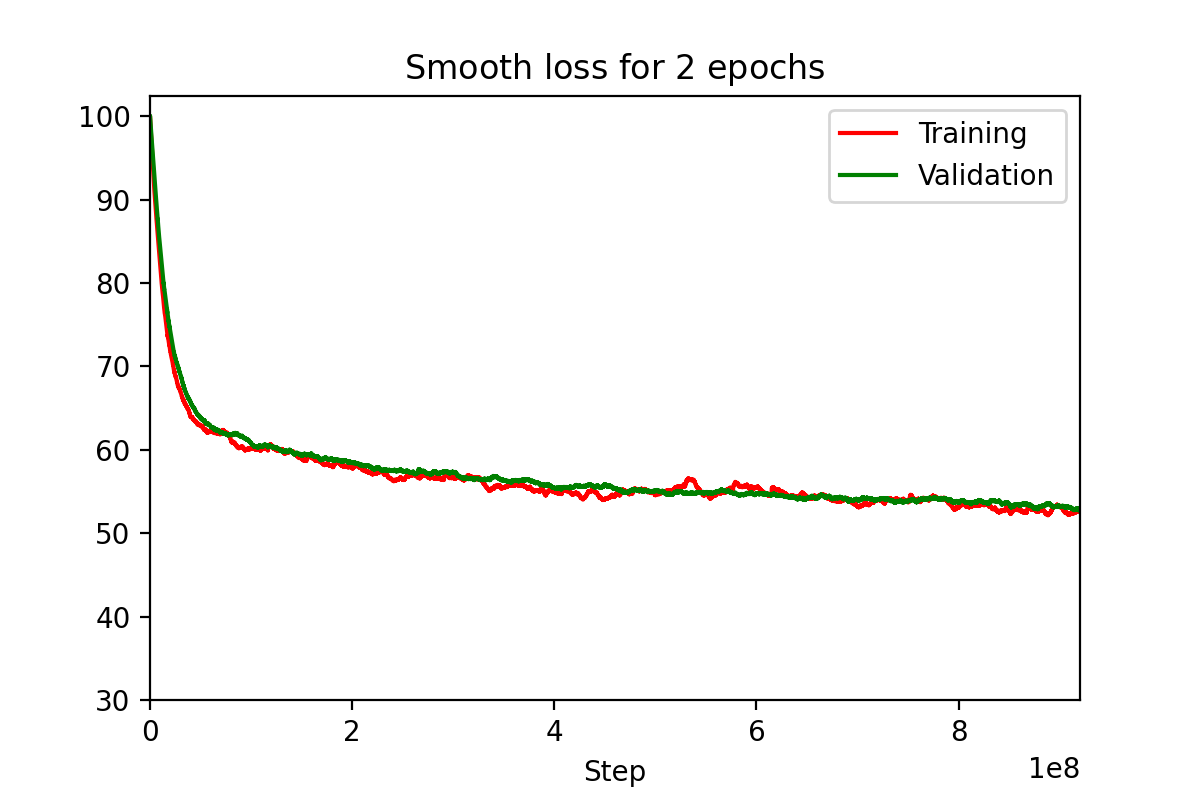
\includegraphics[width=7cm]{../plots/rnn_loss_v1.png}
		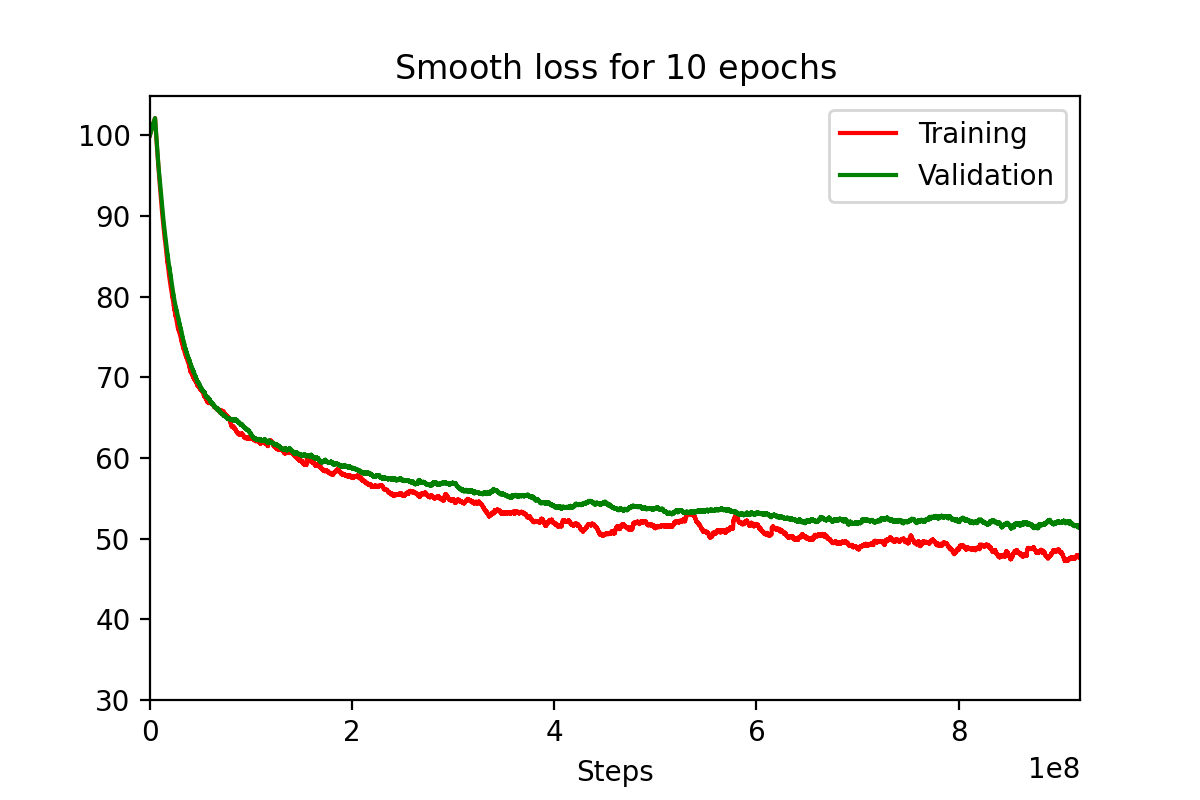
\includegraphics[width=7cm]{../plots/rnn_loss_v2.png}
		\caption{Training and validation loss for \texttt{Adagrad} (left) and \texttt{Adam} (right), after $2$ epochs of training and $\eta = 0.01$.}
 	\end{figure}
	There is a clear distinction between the two optimizers, and the main point seems to be that in this particular example, \texttt{Adam} is more prone to overfitting. The training loss is much lower in the latter case, but the validation loss is very similar. That is, both models seem to be equally good at generalizing to unseen data, while \texttt{Adam} achieves a much lower loss on the training dataset. In fact, the validation loss for \texttt{Adam} seems to increase somewhat towards the end. Hence, in this limited example, \texttt{Adam} does not seem to offer any actual benefit over \texttt{Adagrad}.
	
\newpage
\subsection*{Training with randomly ordered chunks}
	In the first experiment, the data was iterated through sequentially. However, this might introduce temporal dependencies, for example skewing the validation loss whenever we reach the end of an epoch (since the validation loss is extracted as the last $\sim5$\% of sequences. Instead, it seems more sensible to train on randomly selected sequences. This does, however, introduce the problem of memory and context and would require the $h_0$ to be reset at every training step. Thus, I split the data into $100$ blocks, save the last $5$ for validation and shuffle the rest at the beginning of each epoch, such that $h_0$ does not have to be reset at each training step - but instead only at the beginning of each block of training examples. The results are shown for both \texttt{Adagrad} and \texttt{Adam} in the figure below.
	\begin{figure}[h!]
		\centering
		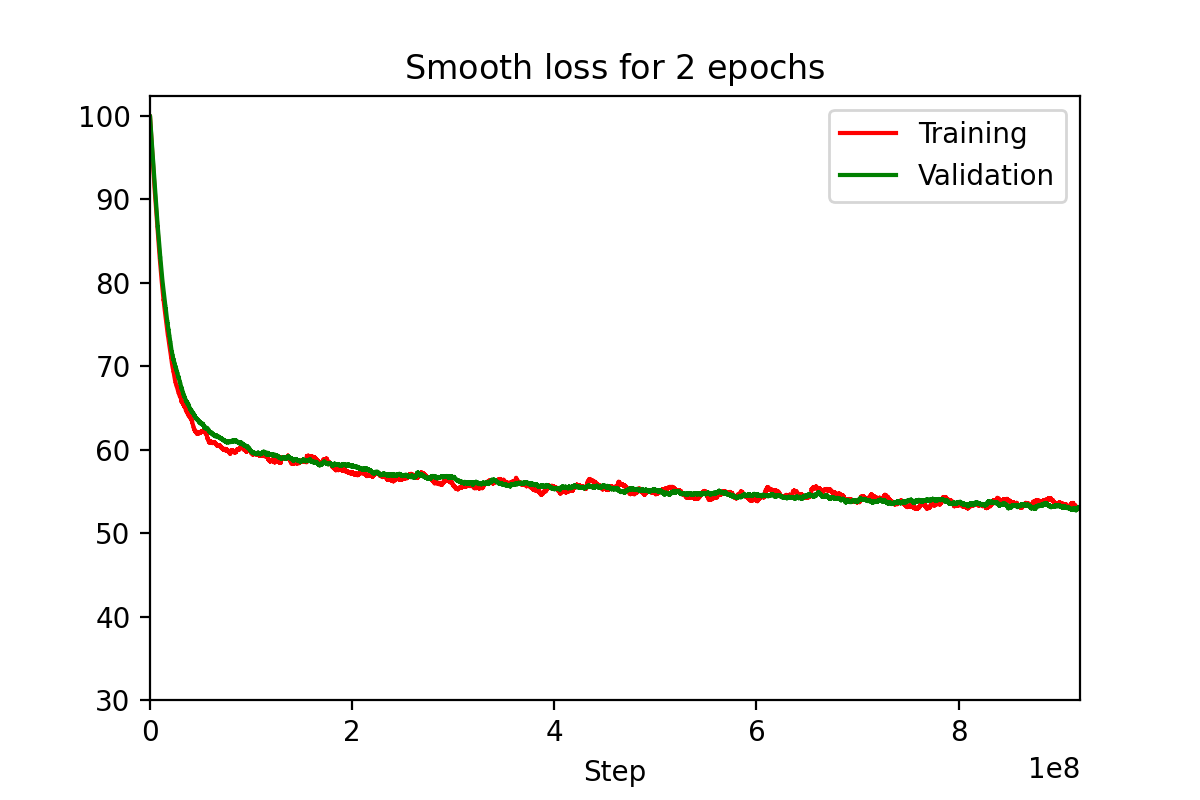
\includegraphics[width=6cm]{../plots/rnn_loss_v3.png}
		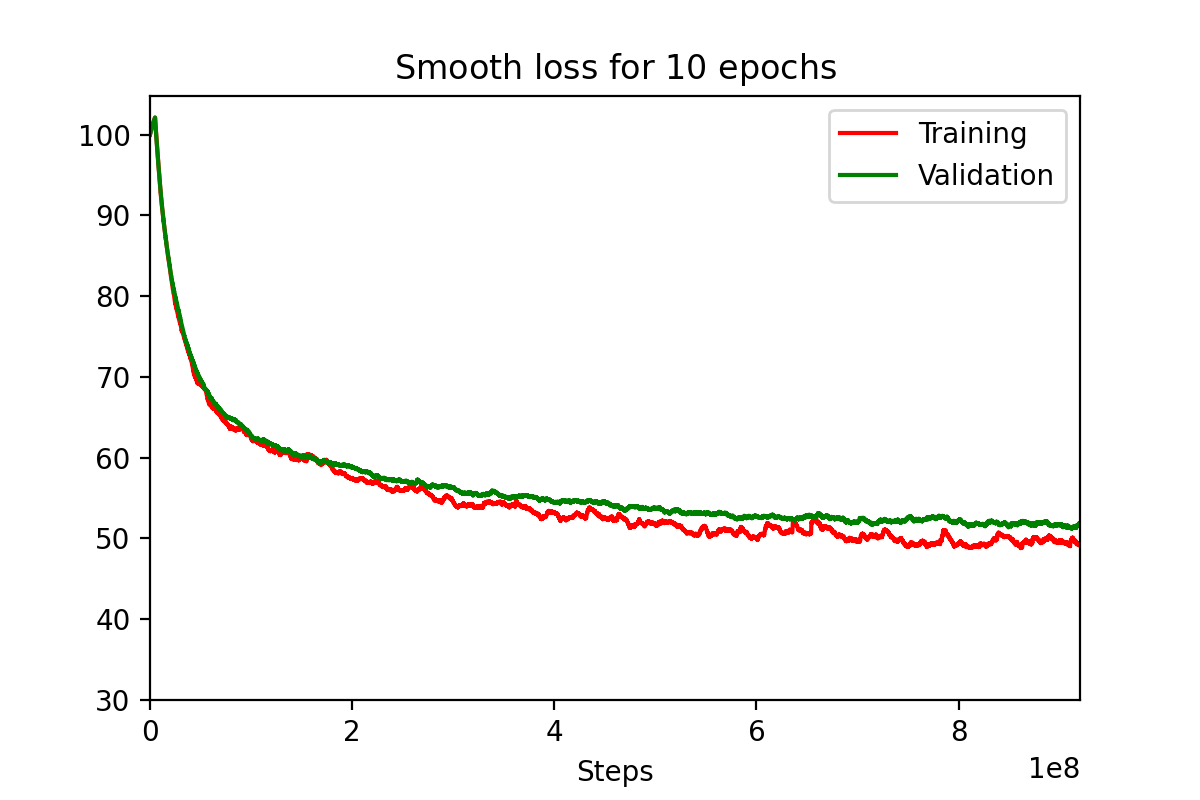
\includegraphics[width=6cm]{../plots/rnn_loss_v4.png}
		\caption{Training and validation loss for \texttt{Adagrad} (left) and \texttt{Adam} (right), after $2$ epochs of training and $\eta = 0.01$ with randomly ordered blocks of training sequences.}
 	\end{figure}
	The results are more or less identical to those obtained without randomly ordered blocks of training sequences. That is, randomizing the sequences does not seem to improve the ability of the model to learn or to generalize significantly much better to new data. In order to possibly improve this, I train another set of models with $T=50$,  $m = 200$, and using \texttt{He} initialization. Further, for the last model with \texttt{Adam}, $t$ is incremented for every second block (rather than at every block). All loss metrics have been normalized with respect to the sequence length to allow for a proper comparison. The results do seem to show that is it possible to achieve a lower loss with the combination of randomized blocks sequences, a wider net, \texttt{He} initialization and a longer sequences, e.g. $T = 50$.
	\begin{figure}[h!]
		\centering
		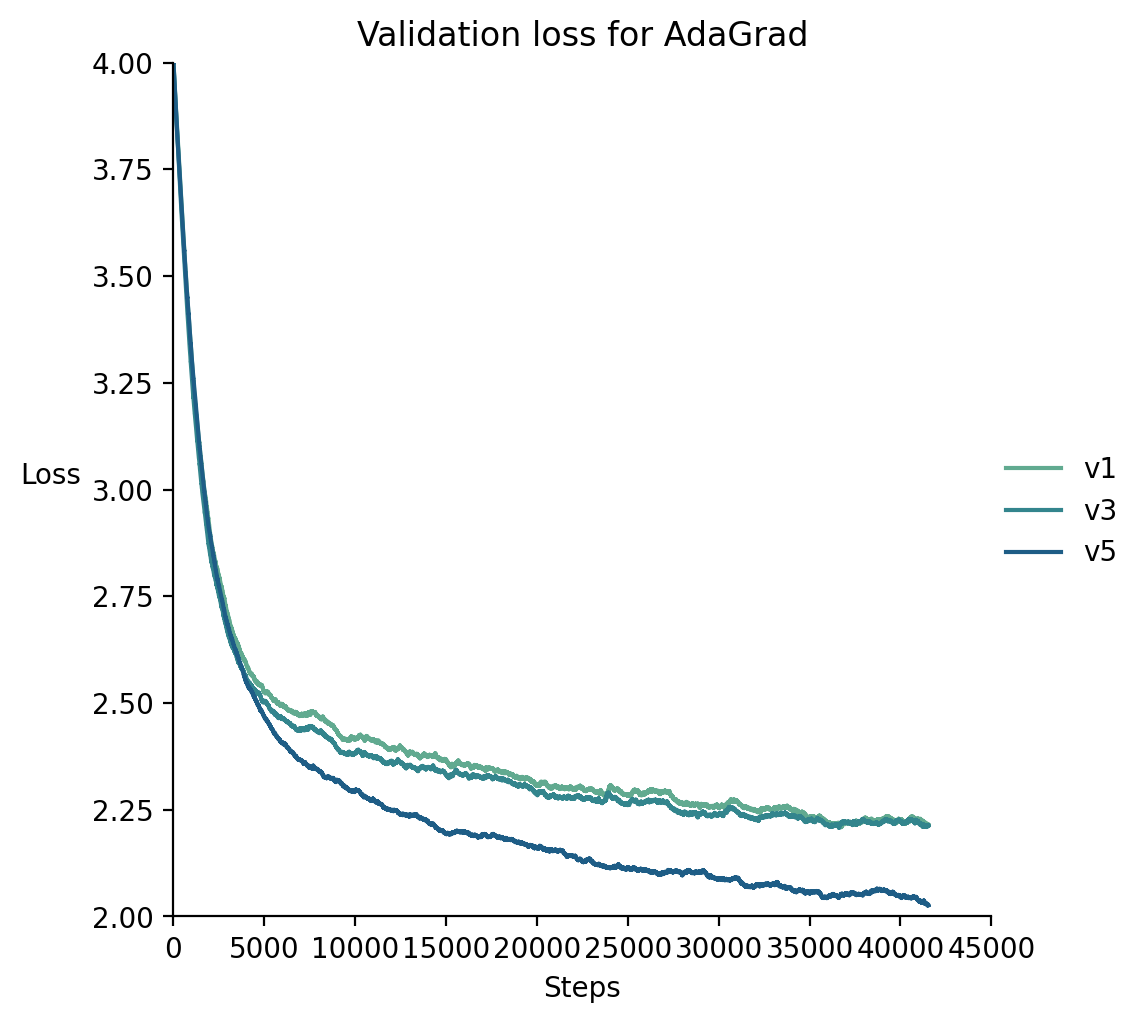
\includegraphics[width=5cm]{../plots/loss_comp_adagrad.png}
		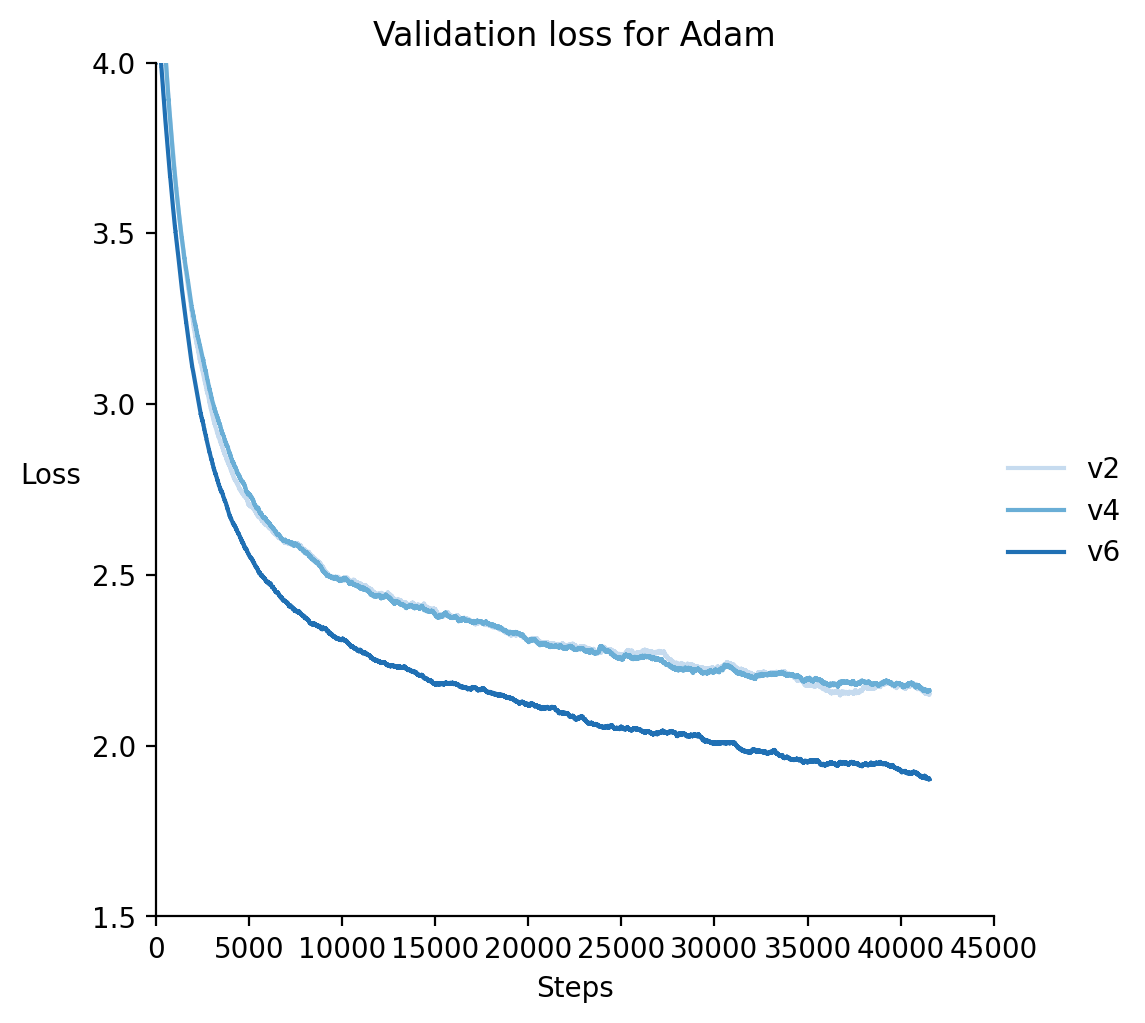
\includegraphics[width=5cm]{../plots/loss_comp_adam.png}
		\caption{Validation loss for models with \texttt{Adagrad} (left) and \texttt{Adam} (right). v1 and v2 are initial models with ordered training sequences, v3 and v4 are trained with randomized blocks with $T = 25$ and $m = 100$. v5 and v6 are trained with $T = 50$, $m = 200$ and with \texttt{He} initialization.}
 	\end{figure}

\newpage
\subsection*{Generating (more) realistic text sequences}
	First, I drew upon the results from the two previous experiments to train a better model. Due to the possible overfitting problems with \texttt{Adam}, I chose to pursue a model similar to v5, using $T=50$, $m=200$, \texttt{He} initialization and a longer training period: $10$ epochs with an \texttt{AdaGrad} optimizer and $\eta = 0.01$. The training results are displayed in the figure below.
	\begin{figure}[h!]
		\centering
		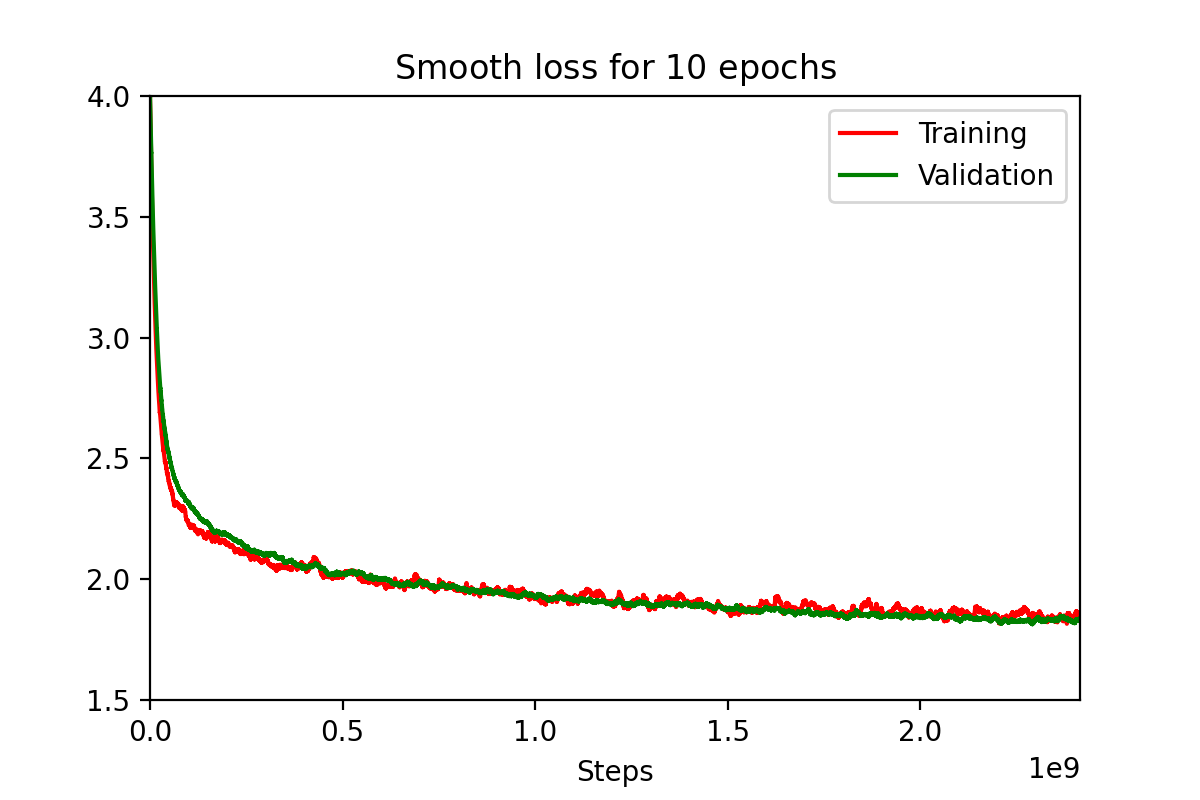
\includegraphics[width=9cm]{../plots/rnn_loss_v7.png}
		\caption{Training and validation loss for \texttt{Adagrad}, after $10$ epochs of training with $\eta = 0.01$, with $T = 50$ and $m = 200$ with \texttt{He} initialization.}
 	\end{figure}
	In what follows, I will display some examples of generated text when using varying temperature values, $\tau$, and varying thresholds, $\theta$. Since the effects $\tau$ and $\theta$ are in a sense proportional - i.e. a high $\theta$ has an effect similar to that of a hihg $\tau$, and vice versa - I have attempted to separate the effects.

\subsection*{Varying $\theta$}
\subsubsection*{$\tau=1.0$, $\theta=1.0$}
	\begin{quote}
		Prgvenscr Potter and to the gtelled the store had sthe ded the sare of the sare goo the squited the start of the tto- he had sof Harry and thing the stareved thee sard.  "I know and in be to the soulang the swat had she roblanging ton the store had Moode the starm pounend the stare 's the stared andi
	\end{quote}

\subsubsection*{$\tau=1.0$, $\theta=0.9$}
	\begin{quote}
		Perthe dol har sere spreton's get, theis hen and tonked eye an the milly - y orared ant her thent bonden me eroce a down courny, and Harry her gails fice foo headed for to ste sivee, you welle way send orfurise, a the seld gooren moven's got dowe inth anothers.  He avery fee sere.\\"No Hormaris.  "Ho 
	\end{quote}

\subsubsection*{$\tau=1.0$, $\theta=0.7$}
	\begin{quote}
		Prtthe don the said to her the tome to do the pouster the camped to his hand the stoply he said and her was a bating and he was stinked to seat the cams of the compinge stad it and stared and Harry was here sood bof the stare the rousher sower stinger, the ground the cange the could be she and the st
	\end{quote}

\subsubsection*{$\tau=1.0$, $\theta=0.5$}
	\begin{quote}
		Prtthe don the said to her the tome to do the pouster the camped to his hand the stoply he said and her was a bating and he was stinked to seat the cams of the compinge stad it and stared and Harry was here sood bof the stare the rousher sower stinger, the ground the cange the could be she and the st
	\end{quote}

\subsection*{Varying $\tau$}
\subsubsection*{$\tau=0.9$, $\theta=0.9$}
	\begin{quote}
		Prgcaniden.  "The doring about to and pistly an the Gobriolly looked all.\\" Ren lonked looked fithor coured you, Hermione thome ther hinge, had tering and way, and Ron facting firming and bagis, with a arling to soupre sach.  Harry capple corit to be hadded has peatering stupe to the wit his mond hi
	\end{quote}

\subsubsection*{$\tau=0.7$, $\theta=0.9$}
	\begin{quote}
		Prrto gaven sumported a thank in ort he to good the nopred the heard for and mearly that could wet stering beand seave sterngs and he there of the fains as the Dark adound in of Mosint, Harry had with as she the bound stere as the said have le to the off corss at a sire beat and to the racked the was
	\end{quote}

\subsubsection*{$\tau=0.5$, $\theta=0.9$}
	\begin{quote}
		Prof sadny, shound a lang that he said the grint of the wiss the sered the call and the was staking the seeped and har been to the cared and the beared somenging as the coully a berting the bating to kis the pond and the grint his panted and the rect a hinge the fored to the tor the dade the stiding
	\end{quote}

\subsection*{Conclusions}
	Varying $\theta$ and $\tau$ clearly have similar effects. As we decrease the parameter values, the generated becomes more "deterministic", and the variation in text decreases rapidly. The model generates fewer special characters and line breaks and the text seems overall to be less "expressive". It seems an "optimal" parameter set is something like $\theta=0.9$, $\tau = 0.7$, in order to generate fairly expressive text containing some keywords and names, such as "Ron", "Hermione", "Harry", and "Potter". However, the larger problem is that the model has a difficult time generating actual words using character sequences. It seems difficult to get more than marginal improvements from more hidden units and longer sequences when employing an RNN. Rather, it might be necessary to extend the model to e.g. an LSTM or a GRU, which is a kind of "simplified" LSTM. It might also be helpful to employ embeddings instead of the sparse categorical inputs attained from one-hot encoding vectors. 
\end{document}